\section{Grundlegende Begriffe und Definitionen}\label{chap:base_theo}

In diesem Kapitel werden die wichtigsten Begriffe für die innerhalb dieser Arbeit vollzogenen Analysen definiert und erläutert.


\subsection{Stromnetz}\label{chap:theo_grid}

Das Stromnetz dient der Übertragung und Verteilung von elektrischer Energie \cite{Paschotta2020}.
Dabei lässt sich das Stromnetz in verschiedene Netzebenen mit jeweils typischen Charakteristika einteilen.
Innerhalb dieses Abschnitts werden diese kurz beschrieben und weitere wichtige Begriffe im Zusammenhang mit Stromnetzen spezifiziert.


\paragraph{Netzebenen:}

Das Stromnetz lässt sich grundsätzlich in Übertragungs- und Verteilnetze unterteilen.
Das Übertragungsnetz dient dem Transport von Strom über lange Strecken bei hohen Spannungen.
Ergänzend erfolgt in den Verteilnetzen die regionale Feinverteilung bei geringeren Spannungen. \cite{Agora2019}\medskip

Innerhalb der Verteilnetze wird zwischen der \glspl{HS}-, \glspl{MS}- und \glspl{NS}-Ebene unterschieden.
Diese Arbeit beschäftigt sich ausschließlich mit den Effekten auf die Verteilnetze auf der \glspl{MS}- und \glspl{NS}-Ebene, inklusive der Umspannebene von \gls{MS} zu \gls{NS}.
In \autoref{tab:Spannungsebenen} finden sich die üblichen Spannungen je Spannungsebene in Deutschland.

{
\renewcommand{\arraystretch}{1.2}% grßerer Zeilenabstand
\sisetup{range-phrase=~bis~}
\begin{table}[H]
	\begin{center}
		\caption{Übliche Spannung und Stromkreislänge der Spannungsebenen im deutschen Verteilnetz}
		\begin{tabu} to 0.65\textwidth {X[0.75] X[1, r] X[1, r]}
			\toprule
            Spannungsebene & Spannung               	& Stromkreislänge   \\\midrule
            Hochspannung   & \SIrange{60}{110}{\kv}     & \SI{95000}{\km}   \\
            Mittelspannung & \SIrange{6}{30}{\kv}  		& \SI{510000}{\km}  \\
            Niederspannung & \SI{230}{\V} 				& \SI{1100000}{\km} \\\bottomrule
            \multicolumn{3}{l}{Quellen: \cite{BDEW2016} und \cite{BMWiNetz}}
		\end{tabu}
		\label{tab:Spannungsebenen}
	\end{center}
	\vspace{-3mm}%Put here to reduce too much white space after your table
\end{table}
}


\paragraph{Netztopologie:}

\gls{NS}-Netze werden in dieser Arbeit als Strahlennetze ausgelegt.
Strahlennetze werden so genannt, da die einzelnen Stränge der Netze strahlenförmig von der \gls{ONS} zu den Endverbrauchern verlaufen.
Vorteil dieser Netzform ist die leichte Berechenbarkeit und die einfache Überwachung des Netzzustandes.
Jedoch führt bereits ein einziger Fehlerfall an einer Einspeisestelle eines Verbrauchers dazu, dass auch alle nachfolgenden Verbraucher vom Netz getrennt werden.
Zudem nimmt der Spannungsabfall über die Länge der Leitung immer weiter zu, wodurch die mögliche Belastbarkeit der Leitung ebenfalls über die Länge abnimmt.

Im Gegensatz zu \gls{NS}-Netzen werden \gls{MS}-Netze als Ringnetze ausgelegt.
Ringnetze bieten den Vorteil, dass diese von zwei Seiten gespeist werden, wodurch eine Ringform entsteht.
Hierdurch können im Falle einer Störung weiterhin alle anderen Verbraucher versorgt werden.
Jedoch werden Ringnetze in der Praxis meist offen betrieben.
Dies bedeutet, dass sich etwa in der Mitte des Rings eine offene Trennstelle befindet.
Auf diese Weise können Ringnetze ebenso einfach überwacht werden wie Strahlennetze.
Im Fehlerfall wird so maximal die Hälfte der Verbraucher vom Netz getrennt.
Durch das Schließen der Trennstelle können dann wieder alle Verbraucher, mit Ausnahme des Fehlerfalls, versorgt werden. \cite{Agora2019} \cite{WNG2020} \cite{Westermann2019}


\paragraph{Gleichzeitigkeit:}

Die Gleichzeitigkeit beschreibt den Anteil der momentan benötigten elektrischen Leistung von der maximalen elektrischen Leistung im Netzgebiet \cite{Agora2019}.
Im Rahmen dieser Arbeit beschreibt die Gleichzeitigkeit in der Regel den Anteil der momentanen elektrischen Last von \glspl{EPKW} im Bezug auf die installierte Leistung von Ladepunkten in einem Netzgebiet.


\paragraph{Elektrische Flexibilität:}

Elektrische Flexibilität beschreibt die Fähigkeit des Stromsystems, trotz einer vorhergesehenen oder unvorhergesehenen Änderung im Verbrauch oder der Erzeugung, einen Ausgleich zwischen Angebot und Nachfrage aufrecht zu erhalten.
Dabei wird die Reaktion des Stromsystems durch ein externes Signal ausgelöst.
Bei dem externen Signal kann es sich beispielsweise um ein Preissignal oder ein physikalisch messbares Signal, wie die Netzfrequenz, handeln.

Elektrische Flexibilität besitzt sowohl eine zeitliche als auch eine geografische Dimension.
Die zeitliche Dimension beschreibt die zeitliche Verschiebung von Last oder Erzeugung und reicht von einer sekündlichen bis zu einer saisonalen Verschiebung.
Unter der geografischen Dimension wird die gemeinsame Nutzung von räumlich verteilten Ressourcen verstanden.
Dabei reicht die räumliche Skala von lokalen Quartierslösungen bis zu internationalen Verbundnetzen. \cite{BNetzA2017} \cite{IEA2014}


\paragraph{Residuallast:}

Die Residuallast beschreibt die Differenz zwischen der benötigten und der erbrachten Leistung von \glspl{FEE} innerhalb eines Betrachtungsgebietes.
Dabei bedeutet eine positive Residuallast, dass der derzeitige Bedarf der Lasten größer ausfällt als die Erzeugung von \glspl{FEE}.
Eine negative Residuallast weist hingegen auf einen Erzeugungsüberschuss hin.
Aufgrund des zunehmenden Anteils von \glspl{FEE} im Stromnetz und der fortschreitenden Sektorkopplung steigt zunehmend die Spreizung zwischen dem maximalen Wert und dem minimalen Wert der Residuallast.

Positive Residuallast wird derzeit zu großen Teilen durch regelbare Kraftwerke gedeckt, während negative Residuallast durch die Abregelung von \glspl{FEE} ausgeglichen wird.
Alternativ kann eine Glättung der Residuallast auch durch die Steuerung von Verbrauchern erreicht werden.
Aufgrund der hohen Ladeleistungen bieten \glspl{EPKW} hierfür ein großes Potential. \cite{Paschotta2020a}


\paragraph{Netzprobleme:}

Netzprobleme sind in dieser Arbeit auf Überlastungen von Betriebsmitteln und Verletzungen des Spannungsbandes bei Endverbrauchern beschränkt.
Bei der Ermittlung von Netzproblemen müssen grundlegend zwei Fälle unterschieden werden.
Im Lastfall überwiegt der Energiebedarf der Verbraucher gegenüber der Energiebereitstellung der Erzeugerkapazitäten im Netzgebiet.
Das Netz muss in diesem Fall in der Lage sein, bereitgestellte Energie aus den überlagerten Netzebenen an die Verbraucher weiterzuleiten.
Im Rückspeisefall überwiegt hingegen die Energiebereitstellung der Erzeugerkapazitäten gegenüber dem Energiebedarf der Verbraucher.
Der erzeugte Strom muss im Rückspeisefall an die überlagerten Netzebenen weitergeleitet werden können.
Verletzungen der thermischen Betriebsmittelbelastungen treten auf, wenn die physikalischen Grenzen von Betriebsmitteln bezüglich ihrer Scheinleistungsbelastbarkeit übertreten werden.
Der Belastungsfaktor eines Betriebsmittels gibt hierbei an, inwieweit ein Betriebsmittel mit Nennscheinleistung belastet werden kann.
Verletzungen des Spannungsbandes sind hingegen als eine unzulässige Abweichung von der Nennspannung bei Endverbrauchern definiert. \cite{Agora2019} \cite{Rehtanz2017}


\subsection{Elektromobilität}

In diesem Kapitel soll auf die wichtigsten Begrifflichkeiten im Zusammenhang mit \glspl{EPKW} eingegangen werden.
Innerhalb dieser Arbeit werden ausschließlich die Auswirkungen der Netzintegration von \glspl{EPKW} untersucht.
Der Einfluss der Elektrifizierung von beispielsweise des öffentlichen Personennahverkehrs, großen betrieblichen Fahrzeugflotten und Lastkraftwagen ist nicht Teil der Erhebungen.


\paragraph{Ladetechnik:}

Die Ladetechnik von \glspl{EPKW} und den korrespondierenden Ladepunkten lässt sich mit Hilfe verschiedener Kriterien klassifizieren.
Die Klassifizierung der Ladetechnik erfolgt innerhalb dieser Arbeit anhand der Höhe ihrer Wirkleistung.
In \autoref{fig:four-quadrant} finden sich die möglichen Betriebszustände der Ladetechnik von \glspl{EPKW} in Abhängigkeit von ihrer \gls{P} und ihrer \gls{Q}.

\begin{figure}[H]
    \centering
    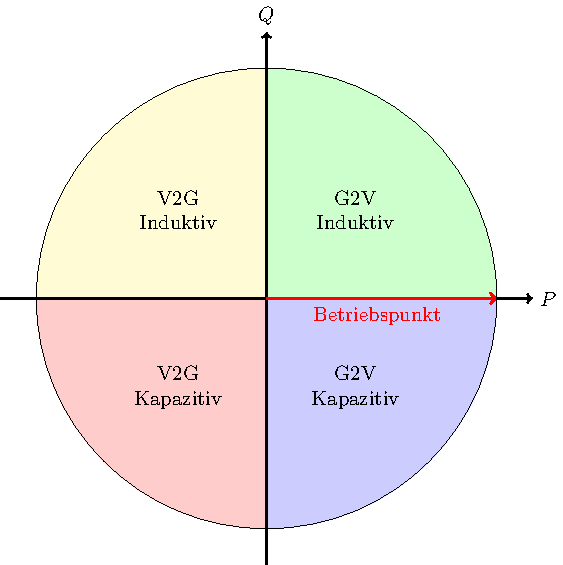
\includegraphics[width=0.7\textwidth]{Bilder/four-quadrant_operation}
    \caption{Mögliche Betriebszustände der Ladetechnik von Elektrofahrzeugen \cite{He2020}}\label{fig:four-quadrant}
\end{figure}

Zusammengefasst werden Ladevorgänge unter der Bezeichnung \gls{G2V}.
Ladevorgänge können sowohl blindleistungsfrei, induktiv oder kapazitiv erfolgen.
In \autoref{fig:four-quadrant} entspricht dieser Modus einer positiven Wirkleistung.
Weiterhin können mit bidirektionaler Ladetechnik \glspl{EPKW} erweiternd entladen werden, um beispielsweise Systemdienstleistungen zu erbringen.
Das gezielte entladen von \glspl{EPKW} wird allgemein unter der Bezeichnung \gls{V2G} zusammengefasst und kann ebenfalls blindleistungsfrei, induktiv oder kapazitiv erfolgen.
In \autoref{fig:four-quadrant} entspricht dieser Modus einer negativen Wirkleistung. \cite{He2020} 
Innerhalb dieser Arbeit erfolgen Ladevorgänge immer blindleistungsfrei, welches dem eingezeichneten Betriebspunkt in \autoref{fig:four-quadrant} entspricht.
Ebenfalls wird der Einsatz von bidirektionaler Ladetechnik nicht untersucht.\medskip

Die einzelnen Ladevorgänge werden anhand ihrer Wirkleistung grob in Normal- und Schnellladevorgänge unterteilt.
Normalladevorgänge finden innerhalb dieser Arbeit bei einer Wirkleistung von maximal \SI{50}{\kw} statt, während Schnellladevorgänge bei einer Leistung von \SIrange[range-phrase=~{oder}~]{150}{350}{\kw} erfolgen.
Dabei wird ein Wirkungsgrad von \SI{90}{\percent} \cite{EliaGroup2020} angenommen.
Eine Übersicht der in dieser Arbeit verwendeten netz- und fahrzeugseitigen Wirkleistungen von Ladepunkten findet sich in \autoref{tab:charging_cap}.
Weiterhin sind die in \autoref{tab:TechPowerCap} zusammengefassten Limitierungen der \glspl{EPKW} zu berücksichtigen.
Unabhängig von der Ladetechnik wird vereinfachend angenommen, dass am Netzverknüpfungspunkt immer eine symmetrische Last anliegt.

{
\renewcommand{\arraystretch}{1.2}% grßerer Zeilenabstand
\sisetup{range-phrase=~bis~}
\begin{table}[H]
	\begin{center}
		\caption{Netz- und fahrzeugseitige Wirkleistung der Ladeinfrastruktur}
		\begin{tabu} to 0.85\textwidth {X[0.5] X[1, r] X[1.1, r]}
			\toprule
			\multicolumn{1}{l}{}           		& Netzseitige Wirkleistung & Fahrzeugseitige Wirkleistung \\ \midrule
			\multirow[t]{4}{*}{Normalladung} 	& \SI{3.7}{\kw}            & \SI{3.3}{\kw}                \\
										   		& \SI{11.0}{\kw}           & \SI{9.9}{\kw}                \\
										   		& \SI{22.0}{\kw}           & \SI{19.8}{\kw}               \\
										   		& \SI{50.0}{\kw}           & \SI{45.0}{\kw}               \\ \midrule
			\multirow[t]{2}{*}{Schnellladung} 	& \SI{150.0}{\kw}          & \SI{135.0}{\kw}              \\
										   		& \SI{350.0}{\kw}          & \SI{315.0}{\kw}              \\ \bottomrule
		\end{tabu}
		\label{tab:charging_cap}
	\end{center}
	\vspace{-3mm}%Put here to reduce too much white space after your table
\end{table}
}


\paragraph{Ladestrategien:}

Ladevorgänge von \glspl{EPKW} können auf Grundlage von unterschiedlichen äußeren Anreizen gesteuert werden.
Grundsätzlich lassen sich hierbei marktorientierte und netzdienliche Ladestrategien unterscheiden.


\subparagraph{Marktorientierte Ladestrategien} haben als Fokus die Minimierung der Kosten für den Strombezug. Dies bedeutet konkret, dass die Ladevorgänge durch ein Preissignal am überregionalen Großhandelsmarkt ausgelöst beziehungsweise unterbrochen werden.
Einerseits führt eine solche Ladestrategie zu einem Ausgleich zwischen Angebot und Nachfrage, da ein hohes Stromangebot zu niedrigen Großhandelsmarktpreisen führt, wodurch das Laden der \glspl{EPKW} ausgelöst wird.
Auf der anderen Seite kann hierdurch die Gleichzeitigkeit erhöht werden, was zu Netzengpässen und zu einem erhöhten lokalen Netzausbaubedarf führen kann.
Somit kann eine marktorientierte Ladestrategie sowohl positive als auch negative Effekte auf das Stromnetz hervorrufen und erfordert einen geeigneten rechtlichen Rahmen. \cite{Agora2019} \cite{Dorendorf2019} \cite{Rehtanz2017}


\subparagraph{Netzdienliche Ladestrategien} setzen hingegen auf die Vermeidung von lokalen Engpässen, welche durch hohe Gleichzeitigkeiten entstehen können.
Hierbei kann zwischen präventiven und aktiven Maßnahmen unterschieden werden.
Präventive Maßnahmen sollen Verbraucher veranlassen, ihre Ladevorgänge in Zeiten geringer, lokaler Netzauslastung zu verlegen.
Dies kann zum Beispiel über monetäre Anreize oder über Quoten erfolgen.
Bei aktiven Maßnahmen handelt es sich hingegen um ein aktives Eingreifen in die Ladevorgänge durch den Netzbetreiber. \cite{Agora2019}


\clearpage
